\documentclass[12pt]{article}

% -----------------------------------------------------------------------------
% Compila no Overleaf com o modelo da SBC: coloque sbc-template.sty e sbc.bst
% na raiz do projeto. Sem eles, o bloco abaixo reproduz margens e cabecalho
% para leitura local.
% -----------------------------------------------------------------------------
\newif\ifthingindexsbc
\IfFileExists{sbc-template.sty}{\thingindexsbctrue}{\thingindexsbcfalse}

\ifthingindexsbc
  \usepackage{sbc-template}
\else
  \usepackage[a4paper,top=3.5cm,bottom=2.5cm,left=3.0cm,right=3.0cm]{geometry}
\fi

\usepackage[utf8]{inputenc}
\usepackage[T1]{fontenc}
\usepackage{textcomp}
\usepackage[brazil,english]{babel}
\usepackage{amsmath}
\usepackage{url}
\usepackage{enumitem}
\usepackage{graphicx}
\usepackage{booktabs}
\usepackage{float}
\usepackage{array}
\usepackage{placeins}
\usepackage{longtable}
% GERADO POR scripts/contagem-testes.sh -- nao edite a mao.
\newcommand{\testesGoArquivos}{157}
\newcommand{\testesGoFuncoes}{717}
\newcommand{\testesIntegracao}{25}
\newcommand{\testesIntegracaoCI}{21}
\newcommand{\testesFrontUnit}{84}
\newcommand{\testesFrontNav}{16}
\newcommand{\testesFrontNavCasos}{33}
\newcommand{\coberturaBackend}{56,2}

\hyphenation{Thing-Index}

% Repositorio com os anexos (diagramas, telas, tabelas completas).
\newcommand{\repositorio}{\url{https://github.com/EduardoMG12/ThingIndex}}

% Deixa tabelas perto de onde sao citadas, em vez de irem para o fim.
\renewcommand{\topfraction}{0.9}
\renewcommand{\bottomfraction}{0.8}
\renewcommand{\textfraction}{0.07}
\renewcommand{\floatpagefraction}{0.75}
\setcounter{totalnumber}{4}

% Citacao so com o ano, para frases que ja nomeiam o autor ("Codd [1970]").
% O sbc.bst grava o rotulo como "Autor Ano": o ano sao os 4 ultimos
% caracteres. Na primeira compilacao, antes do .aux, sai "[?]".
\makeatletter
% Remove palavras ate sobrar a ultima (o ano). #2 vazio = acabou.
\def\thingindex@ultima#1 #2\@nil{\if\relax\detokenize{#2}\relax #1\else\thingindex@ultima#2\@nil\fi}
\newcommand{\citeyear}[1]{%
  \if@filesw\immediate\write\@auxout{\string\citation{#1}}\fi
  \@ifundefined{b@#1}{[?]}{[\expandafter\expandafter\expandafter\thingindex@ultima\csname b@#1\endcsname{} \@nil]}}
\makeatother

\ifthingindexsbc\else
  \makeatletter
  \newcommand{\inst}[1]{}
  \newcommand{\thingindex@address}{}
  \newcommand{\address}[1]{\gdef\thingindex@address{#1}}
  \newcommand{\email}[1]{\texttt{#1}}
  \renewcommand{\maketitle}{
    \begin{center}
      {\bfseries\LARGE \@title\par}
      \vspace{12pt}
      {\normalsize\bfseries \@author\par}
      \vspace{12pt}
      {\normalsize \thingindex@address\par}
    \end{center}
    \vspace{12pt}
  }
  \newenvironment{resumo}
    {\begin{quote}\noindent\textbf{Resumo. }}
    {\end{quote}}
  \renewenvironment{abstract}
    {\begin{quote}\noindent\textbf{Abstract. }}
    {\end{quote}}
  \makeatother
\fi

\sloppy
\setlist[itemize]{leftmargin=1.5em}
\setlist[enumerate]{leftmargin=1.8em}

\title{ThingIndex: Inteligência Documental com Proveniência\\ Verificável sobre Modelo Relacional}

\author{Charles Eduardo Mello Guimarães\inst{1}}

\address{
  Instituto Federal do Paraná (IFPR) -- Campus Palmas\\
  Curso de Sistemas de Informação\\
  Palmas -- PR -- Brasil\\
  \email{charles.eduardo.mello.guimaraes@hotmail.com}
}

\begin{document}

\maketitle

\selectlanguage{brazil}
\begin{resumo}
Quem consulta acervos normativos precisa de respostas que possam ser conferidas no original. Por \emph{Design Science Research}, construiu-se e avaliou-se o ThingIndex, que guarda PDFs em tabelas relacionais, com a coordenada de origem exigida por chave estrangeira, recupera trechos por BM25 e mostra documento, página e região de cada fonte. Em três acervos públicos (leis, normas e manuais) com perguntas escritas depois do desenvolvimento, a taxa de acerto foi de 0,695 com a pergunta original e de 0,887 com expansão experimental da pergunta pelo mesmo LLM ($p < 0{,}001$). No acervo de desenvolvimento, o sistema usou 1/26 dos \emph{tokens} do documento inteiro (mediana). A fonte verificável não impediu o pior erro: citar corretamente uma lei revogada.
\end{resumo}

\noindent\textbf{Palavras-chave}: recuperação de informação, proveniência de dados, geração aumentada por recuperação, modelagem relacional, \emph{Design Science Research}.

\selectlanguage{english}
\begin{abstract}
People who consult regulatory collections need answers they can check against the original. Following Design Science Research, this work built and evaluated ThingIndex, which stores PDFs in relational tables, with the source coordinate enforced by a foreign key, retrieves passages with BM25 and shows each source's document, page and region. On three public collections (laws, regulations and manuals) with questions written after development, accuracy was 0.695 with the original question and 0.887 with experimental query expansion by the same LLM ($p < 0.001$). On the development collection it used a median of 1/26 of the whole-document tokens. A verifiable source does not prevent the worst error observed: correctly citing a law that has been repealed.
\end{abstract}

\noindent\textbf{Keywords}: information retrieval, data provenance, retrieval-augmented generation, relational modeling, design science research.

\selectlanguage{brazil}

% =============================================================================
% 1. INTRODUCAO
% =============================================================================
\section{Introdução}
\label{sec:introducao}

Muitas perguntas de trabalho têm resposta em um documento que já existe. Um servidor do setor de compras de uma prefeitura precisa saber se a modalidade ``tomada de preços'' ainda pode ser usada; um técnico de segurança do trabalho precisa confirmar quem paga o equipamento de proteção; uma secretaria acadêmica precisa localizar a carga horária de um curso no projeto pedagógico. A resposta está em leis, normas e regulamentos, que costumam ficar em pastas compartilhadas ou em sistemas que indexam o nome e os metadados do arquivo, mas não o conteúdo~\cite{schymik2015benefits}. Achar a cláusula exige abrir o arquivo certo e lê-lo, e uma resposta errada vira retrabalho ou decisão mal fundamentada.

Os modelos de linguagem de grande escala (LLMs), como os que estão por trás dos assistentes de conversa, mudaram a expectativa: em vez de uma lista de arquivos, espera-se uma resposta pronta. A arquitetura mais usada para isso é a geração aumentada por recuperação (RAG): antes de responder, o sistema busca trechos relevantes nos documentos e os entrega ao modelo junto com a pergunta~\cite{lewis2020rag}. Para quem responde por uma decisão, porém, a resposta só tem valor se puder ser conferida no original. Uma resposta correta sem a página de origem obriga o leitor a refazer a busca, e uma resposta errada com uma citação plausível tende a passar despercebida.

Neste trabalho, uma fonte é \emph{auditável} quando aponta documento, página e região de onde veio, e essa coordenada vem do banco de dados, e não do texto escrito pelo modelo. Na literatura de bancos de dados, isso se chama proveniência \emph{where}~\cite{buneman2001provenance}. A pergunta de pesquisa é: \emph{unidades estruturais de PDFs persistidas em modelo relacional, com a coordenada de origem garantida pelo esquema e recuperadas por um método lexical, bastam para um sistema de perguntas e respostas cujas fontes possam ser conferidas no original?}

Para responder, foi construído o ThingIndex. O sistema extrai a estrutura dos PDFs (páginas, parágrafos com posição, tabelas e sumário), guarda essa estrutura em tabelas do PostgreSQL, busca os trechos por palavras, com o algoritmo BM25, e devolve com cada fonte a coordenada que permite abri-la no documento. O LLM só entra no final, para redigir a resposta a partir das fontes encontradas. Não usar um banco vetorial, que é a escolha mais comum em RAG, foi uma decisão de projeto, tomada por simplicidade de operação e para que a mesma pergunta traga sempre as mesmas fontes; a Seção~\ref{sec:resultados} mede o que essa decisão custa.

As contribuições são:
\begin{enumerate}
  \item o sistema, implementado e testado, em que a coordenada de origem de cada unidade recuperável é exigida por chave estrangeira e conferida por teste;
  \item um protocolo de avaliação que dificulta resultados favoráveis por construção: hipóteses registradas antes de medir, gabaritos travados por \emph{hash}, perguntas em pares (com as palavras do documento e com outras palavras) e registro das correções feitas depois de medir;
  \item resultados em português, em sete acervos, sobre acerto, origem das fontes e custo, incluindo um erro que a fonte verificável não detecta: a resposta que cita corretamente uma norma revogada.
\end{enumerate}

O texto segue esta ordem: objetivos (Seção~\ref{sec:objetivos}), referencial teórico (Seção~\ref{sec:referencial}), trabalhos relacionados (Seção~\ref{sec:relacionados}), metodologia (Seção~\ref{sec:metodologia}), o sistema (Seção~\ref{sec:artefato}), o desenho da avaliação (Seção~\ref{sec:avaliacao}), os resultados (Seção~\ref{sec:resultados}), a discussão (Seção~\ref{sec:discussao}) e a conclusão (Seção~\ref{sec:conclusao}). Diagramas, telas e tabelas completas estão no repositório do projeto (Apêndice~A).

% =============================================================================
% 2. OBJETIVOS
% =============================================================================
\section{Objetivos}
\label{sec:objetivos}

O objetivo geral é projetar, implementar e avaliar o ThingIndex, um sistema de inteligência documental que organiza e recupera o conteúdo de coleções de PDFs com fontes verificáveis, e comparar sua recuperação com alternativas densas e com a entrega do documento inteiro a um LLM.

Os objetivos específicos são:
\begin{enumerate}
  \item modelar em tabelas relacionais as estruturas extraídas de PDFs (páginas, parágrafos, tabelas, sumário e trechos), com a coordenada de origem de cada unidade exigida pelo esquema;
  \item implementar o sistema completo, com indexação assíncrona resiliente a falhas, recuperação por coleção e \emph{chat} que exibe as fontes;
  \item definir métricas de auditabilidade e um protocolo de avaliação com gabaritos independentes da saída do sistema;
  \item comparar a recuperação lexical com a densa, exata e aproximada, em qualidade de ordenação num \emph{corpus} de controle e em estabilidade;
  \item comparar, em acerto, proveniência e custo, o contexto recuperado com a entrega do documento inteiro ao modelo;
  \item medir o sistema em acervos de domínios distintos e testar intervenções dirigidas às causas de erro encontradas.
\end{enumerate}

% =============================================================================
% 3. REFERENCIAL TEORICO
% =============================================================================
\section{Referencial Teórico}
\label{sec:referencial}

Esta seção apresenta só os conceitos de que o restante do texto depende. A Tabela~\ref{tab:glossario} resume os termos mais usados, para consulta durante a leitura.

\begin{table}[!htbp]
\centering
\caption{Termos usados no artigo, no sentido em que são usados aqui.}
\label{tab:glossario}
\small
\begin{tabular}{p{3.3cm}p{10.2cm}}
\toprule
Termo & Significado \\
\midrule
LLM & Modelo de linguagem de grande escala: o modelo que lê um texto de entrada (o \emph{prompt}) e escreve a resposta. \\
\emph{Token} & Pedaço de palavra que o LLM processa. O custo de uma chamada é proporcional aos \emph{tokens} enviados. \\
RAG & Geração aumentada por recuperação: buscar trechos nos documentos e entregá-los ao LLM junto com a pergunta. \\
Busca lexical & Busca por palavras: um trecho é bom se contém as palavras da pergunta. O BM25 é o algoritmo usado. \\
Busca densa & Busca por significado: pergunta e trecho viram vetores de números, e trechos de sentido parecido ficam próximos. \\
Índice aproximado & Estrutura que acelera a busca densa olhando só parte dos vetores, ao custo de às vezes perder o mais próximo (IVF e HNSW). \\
Unidade, trecho & Unidade é cada parte do PDF guardada numa linha de tabela (página, parágrafo, linha de tabela, seção). Trecho é um grupo de parágrafos de uma seção, citado como fonte. \\
Proveniência \emph{where} & Saber de onde um dado veio: aqui, documento, página e região do PDF. \\
Braço & Cada configuração comparada num experimento (por exemplo, BM25 contra busca densa). \\
Gabarito & Lista de perguntas, cada uma com a página onde está a resposta e o padrão que uma resposta certa precisa conter. \\
Literal e paráfrase & As duas redações de uma mesma pergunta: com as palavras do documento e com as palavras de quem não leu o documento. \\
\bottomrule
\end{tabular}
\end{table}

\subsection{Inteligência documental}
\label{sec:ref-conhecimento}

Nonaka e Takeuchi~\citeyear{nonaka1995knowledge} distinguem o conhecimento tácito, que está nas pessoas, do explícito, registrado em documentos. O explícito só é reaproveitado se puder ser encontrado e recombinado, e Davenport e Prusak~\citeyear{davenport1998working} argumentam que o valor do conhecimento de uma organização depende disso. Chama-se aqui de \emph{inteligência documental} a capacidade de um sistema extrair, organizar e recuperar conhecimento a partir do conteúdo dos documentos, e não só do nome e dos metadados. No ThingIndex, isso significa tratar o PDF como um conjunto de unidades endereçáveis (a página, o parágrafo, a linha de tabela), cada uma com uma posição conhecida no original.

\subsection{Busca por palavras e busca por significado}
\label{sec:ref-ri}

A recuperação de informação estuda como encontrar, numa coleção, os itens que atendem a uma necessidade de informação~\cite{manning2008ir}. A forma mais antiga é a busca por palavras, ou \emph{lexical}. O BM25, usado no ThingIndex, dá uma nota a cada trecho a partir de três ideias~\cite{robertson2009bm25}: cada palavra da pergunta encontrada no trecho soma pontos; uma palavra rara na coleção vale mais que uma comum, porque diz mais sobre o assunto (num acervo de normas de segurança, ``EPI'' vale mais que ``trabalho''); e repetir a palavra ajuda cada vez menos, enquanto trechos longos são penalizados, para que um trecho não vença só por ter mais palavras. Os parâmetros $k_1$ e $b$ regulam essas duas últimas ideias. A ideia de dar mais peso à palavra rara já estava no modelo clássico TF-IDF~\cite{salton1989automatic}; a primeira versão do ThingIndex não a usava e só contava ocorrências. O BM25 é simples e difícil de superar: num conjunto de testes em domínios variados, o BEIR, ele foi melhor que a maior parte dos métodos densos da época~\cite{thakur2021beir}.

A fraqueza da busca por palavras é o descasamento de vocabulário. Furnas et al.~\citeyear{furnas1987vocabulary} mostraram que duas pessoas raramente escolhem a mesma palavra para a mesma coisa: quem pergunta ``quem paga o capacete e a luva?'' não usa as palavras da norma, que fala em equipamento de proteção individual. Uma solução é a \emph{expansão da pergunta}, que acrescenta à consulta termos relacionados~\cite{carpineto2012survey}. Com LLMs, pode-se pedir ao próprio modelo esses termos, que é o método de Jagerman et al.~\citeyear{jagerman2023qe} e o usado neste trabalho. O ganho, porém, não é garantido: comparando várias técnicas, Weller et al.~\citeyear{weller2024expansion} observaram que a expansão ajuda os recuperadores mais fracos e pode atrapalhar os mais fortes.

A outra família é a busca \emph{densa}, ou por significado. Um modelo treinado converte cada texto numa lista de centenas de números, chamada vetor, de modo que textos de sentido parecido fiquem com vetores próximos~\cite{karpukhin2020dense}. A pergunta também vira vetor, e a busca devolve os trechos mais próximos dela. A vantagem é encontrar ``carro'' quando se pergunta ``automóvel''. Este trabalho usa o modelo \texttt{multilingual-e5-base}~\cite{wang2024me5}, um modelo multilíngue que gera vetores de 768 números.

Comparar a pergunta com todos os vetores guardados é exato, mas fica lento com milhões deles. Por isso se usam \emph{índices aproximados}. O IVF separa os vetores em grupos, como gavetas, e na consulta abre só as gavetas mais próximas~\cite{jegou2011product}; o HNSW liga cada vetor a seus vizinhos num grafo e caminha por ele até a região da pergunta~\cite{malkov2020hnsw}. Os dois podem deixar de fora um vizinho que a busca exata acharia. A extensão pgvector, que acrescenta esses índices ao PostgreSQL, avisa na documentação que o índice aproximado pode devolver resultados diferentes dos da busca exata~\cite{pgvector2026}. Para um sistema que precisa trazer sempre as mesmas fontes, essa variação importa, e a Seção~\ref{sec:res-determinismo} mede quando ela acontece.

Por fim, listas de resultados de métodos diferentes podem ser combinadas pela fusão por posição recíproca (RRF), que soma o inverso da posição de cada item em cada lista~\cite{cormack2009rrf}. Isso permite misturar a busca por palavras com a densa sem precisar comparar as notas de cada uma.

\subsection{Geração aumentada por recuperação}
\label{sec:ref-rag}

Um LLM responde a partir do que viu no treinamento e, sem uma fonte externa, produz com frequência afirmações fluentes e falsas, o que se chama de alucinação~\cite{ji2023survey}. A RAG, proposta por Lewis et al.~\citeyear{lewis2020rag}, combina um buscador com o gerador: os trechos encontrados entram no \emph{prompt} junto com a pergunta, e o modelo é instruído a responder a partir deles. Na forma mais comum, os documentos são cortados em blocos de tamanho fixo, convertidos em vetores e guardados num banco vetorial~\cite{gao2023ragsurvey}. Nesse corte, a ligação de cada bloco com a página do original fica a cargo de quem monta o sistema.

Três resultados recentes mostram os limites dessa arquitetura e aparecem nos experimentos deste trabalho. O modelo aproveita pior a informação que está no meio de um texto longo~\cite{liu2024lost}, o que pesa contra entregar documentos inteiros. Quando as fontes entregues se contradizem, como uma lei e a lei que a revogou, o modelo não resolve o conflito de forma confiável~\cite{xu2024knowledge}. E o modelo tende a concordar com a premissa da pergunta mesmo quando ela é falsa, comportamento chamado de bajulação~\cite{sharma2024sycophancy}. Com modelos que aceitam textos muito longos, uma alternativa à RAG é entregar o documento inteiro; Li et al.~\citeyear{li2024ragorlc} compararam as duas estratégias e concluíram que o documento inteiro acerta mais quando há recursos para ele, e a recuperação custa muito menos.

\subsection{Modelo relacional e proveniência}
\label{sec:ref-relacional}

No modelo relacional de Codd~\citeyear{codd1970}, os dados ficam em tabelas, e as ligações entre elas são garantidas por chaves: uma chave estrangeira faz o banco recusar uma linha que aponte para outra que não existe. Transações garantem que um conjunto de escritas aconteça por inteiro ou não aconteça~\cite{date2004introduction}. Essas garantias são do banco, e não dependem de o programa lembrar de cumpri-las.

Proveniência é a informação sobre a origem de um dado. Buneman et al.~\citeyear{buneman2001provenance} distinguem a proveniência \emph{where}, que diz onde está o valor de origem, da \emph{why}, que diz quais dados justificam um resultado. No ThingIndex, o interesse é a \emph{where}: cada unidade recuperada aponta documento, página e região. Como as unidades são linhas de tabela, o próprio esquema pode exigir essa coordenada.

É preciso separar isso de outra pergunta: a frase da resposta é sustentada pela fonte citada? Essa é a noção de \emph{atribuição}~\cite{rashkin2023attribution}. Ao auditar quatro buscadores generativos comerciais, Liu et al.~\citeyear{liu2023verifiability} encontraram só 51,5\% das frases integralmente apoiadas pelas citações. A proveniência garantida pelo esquema é condição para conferir a atribuição, mas não a substitui: o sistema pode apontar a página certa de um trecho que não sustenta o que a resposta diz.

\subsection{Integração assíncrona}
\label{sec:ref-integracao}

Indexar um PDF leva tempo, então o envio só registra o pedido, e um processo separado faz o trabalho depois, avisado por uma fila de mensagens. O problema é que gravar no banco e publicar na fila são duas escritas sem transação comum: se o sistema cair entre elas, o documento fica registrado sem que ninguém seja avisado. O padrão \emph{transactional outbox} resolve isso gravando a mensagem numa tabela, na mesma transação do registro, e publicando-a depois~\cite{richardson2018microservices}. Mensagens que falham repetidamente vão para uma fila separada, a de mensagens mortas, onde podem ser examinadas sem travar as demais~\cite{hohpe2003eip}.

% =============================================================================
% 4. TRABALHOS RELACIONADOS
% =============================================================================
\section{Trabalhos Relacionados}
\label{sec:relacionados}

A Tabela~\ref{tab:relacionados} compara o ThingIndex com os trabalhos mais próximos quanto a duas escolhas: como as fontes são escolhidas e de onde vem a indicação de origem que o usuário vê.

\begin{table}[!htbp]
\centering
\caption{Comparação com trabalhos relacionados.}
\label{tab:relacionados}
\small
\begin{tabular}{p{3.0cm}p{5.0cm}p{5.5cm}}
\toprule
Trabalho & Como escolhe as fontes & Origem da fonte \\
\midrule
LangChain~\cite{langchain2022}, LlamaIndex~\cite{llamaindex2022} & Bibliotecas: o desenvolvedor escolhe o corte em blocos e o buscador & Os metadados que o desenvolvedor anexar ao bloco \\
GraphRAG~\cite{edge2024graphrag} & Grafo de entidades e resumos construídos por LLM & Resumos gerados, e não o texto original \\
RAPTOR~\cite{sarthi2024raptor} & Árvore de resumos sobre os blocos & Resumos gerados em vários níveis \\
PageIndex~\cite{pageindex2025} & O LLM navega a árvore de seções do PDF & A seção escolhida pelo modelo; sem avaliação publicada \\
Assistentes comerciais & Fechado & Referência ao documento, sem garantia que se possa inspecionar \\
ThingIndex & BM25 sobre unidades guardadas em tabelas; nenhum modelo escolhe as fontes & Documento, página e região lidos do banco e exigidos por chave estrangeira \\
\bottomrule
\end{tabular}
\end{table}

As bibliotecas LangChain e LlamaIndex servem para montar aplicações com LLMs e deixam a proveniência a cargo de quem as usa; o ThingIndex é uma aplicação completa que fixa uma escolha (unidades estruturais com coordenada) e a avalia. O GraphRAG e o RAPTOR miram perguntas que exigem visão de conjunto do acervo, mas dependem do LLM já na indexação, e o que recuperam pode ser um resumo gerado. O PageIndex é a motivação mais próxima: também usa a estrutura do PDF e dispensa vetores, mas é o modelo que escolhe a seção. Assistentes comerciais que aceitam PDFs escalam e atendem várias pessoas, o que o ThingIndex não faz; ele difere deles por poder rodar inteiramente na instalação da organização, com um modelo aberto, e por ter a garantia de proveniência visível no esquema e no código. Não houve comparação experimental com esses produtos nem com o PageIndex.

Quanto à avaliação, o BEIR~\cite{thakur2021beir} mostrou que medir recuperação num só domínio superestima os métodos; o RAGAS~\cite{es2024ragas} usa o próprio LLM como juiz das respostas; e o ALCE~\cite{gao2023alce} mede se as citações sustentam o texto. Este trabalho preferiu gabaritos escritos à mão, com página-alvo e padrão de resposta, para que o juiz não seja outro modelo. Os trabalhos acima ou propõem ferramentas sem avaliar a proveniência, ou avaliam a atribuição sem tratar de como a coordenada é guardada. Este trabalho junta as duas coisas num sistema completo, medido em documentos reais em português.

% =============================================================================
% 5. METODOLOGIA
% =============================================================================
\section{Metodologia}
\label{sec:metodologia}

O trabalho é uma pesquisa aplicada conduzida segundo a \emph{Design Science Research} (DSR), em que se constrói um artefato para resolver um problema relevante e se avalia o artefato com rigor~\cite{hevner2004design}. Seguiu-se o processo de seis atividades de Peffers et al.~\citeyear{peffers2007design}:

\begin{enumerate}
  \item \textbf{Identificação do problema}: consulta a acervos normativos sem fonte verificável (Seção~\ref{sec:introducao}). Não houve levantamento com usuários; o problema foi caracterizado por casos de uso típicos e pela literatura.
  \item \textbf{Objetivos da solução}: recuperar trechos com coordenada de origem garantida pelo esquema, com custo por pergunta que não cresça com o tamanho do documento (Seção~\ref{sec:objetivos}).
  \item \textbf{Projeto e desenvolvimento}: o ThingIndex (Seção~\ref{sec:artefato}).
  \item \textbf{Demonstração}: uso sobre seis acervos de PDFs reais e um \emph{corpus} sintético de controle (Seção~\ref{sec:avaliacao}).
  \item \textbf{Avaliação}: experimentos de recuperação, de origem das fontes e de geração da resposta (Seção~\ref{sec:resultados}). A utilidade para usuários finais não foi avaliada.
  \item \textbf{Comunicação}: este artigo e o repositório do projeto, com código, dados e \emph{scripts} de análise.
\end{enumerate}

O desenvolvimento foi feito em ciclos: cada experimento que revelava uma limitação gerava uma mudança no sistema, medida no ciclo seguinte. Esses ciclos usaram um único acervo, o de ensino, que por isso funcionou como \emph{conjunto de desenvolvimento}: o sistema foi ajustado olhando para as suas 72 perguntas, e seus resultados tendem a ser otimistas. Os gabaritos dos demais acervos foram escritos depois, sobre documentos ainda não usados, e funcionam como \emph{conjunto de teste}. Para evitar que os ciclos produzissem bons números por construção, quatro práticas foram adotadas:
\begin{itemize}
  \item \textbf{Pré-registro}: nas duas intervenções testadas (Seções~\ref{sec:res-enriquecimento} e~\ref{sec:res-expansao}), a hipótese, o critério de sucesso e a análise foram escritos e versionados antes do código.
  \item \textbf{Gabaritos travados}: cada gabarito registra o \emph{hash} SHA-256 do seu conteúdo, e o programa de avaliação recusa um gabarito alterado sem atualizar o \emph{hash}, o que deixa toda alteração visível no histórico.
  \item \textbf{Números gerados por \emph{script}}: os resultados ficam em arquivos CSV, uma linha por pergunta e repetição, e as tabelas do artigo são geradas ou conferidas a partir deles.
  \item \textbf{Registro das correções feitas depois de medir}: toda alteração de gabarito ou de critério feita depois de uma medição foi registrada com data, motivo e efeito nos números, no arquivo \texttt{docs/article/results/alteracoes-pos-medicao.md}. As que mudam números deste artigo são citadas onde o número aparece.
\end{itemize}

% =============================================================================
% 6. O ARTEFATO
% =============================================================================
\section{O ThingIndex}
\label{sec:artefato}

\subsection{Requisitos}
\label{sec:requisitos}

São doze requisitos funcionais, cada um ligado a rotas da API cobertas por testes automatizados: cadastro e autenticação; organização em categorias e coleções; envio de documentos (PDF, HTML e planilha); indexação assíncrona; enriquecimento opcional por LLM; recuperação de contexto por API; \emph{chat} com as fontes citadas; abertura de cada fonte na página e na região de origem; configuração de provedores de LLM e de armazenamento com credencial cifrada; acompanhamento de \emph{tokens} e custo; trilha de auditoria; e reprocessamento de falhas. A lista com a rota de cada requisito e o diagrama de casos de uso estão no repositório (Apêndice~A).

Os principais requisitos não funcionais são: integridade referencial e transações no armazenamento da estrutura extraída; separação em camadas; segurança (senha com bcrypt, sessão por \emph{token} JWT, credencial de provedor cifrada com AES-GCM e limite de requisições nas rotas de autenticação, envio e \emph{chat}); execução reproduzível por Docker Compose; e recuperação determinística, isto é, a mesma pergunta sobre o mesmo índice traz as mesmas fontes na mesma ordem. Quanto à privacidade, com um modelo rodando na própria instalação nenhum conteúdo sai dela; com um provedor externo, a pergunta e os trechos recuperados são enviados a ele, e cabe à organização a base legal para isso, nos termos da Lei Geral de Proteção de Dados (LGPD). Nesta versão o sistema é de uso individual: acervo, credenciais e histórico pertencem a um usuário, sem compartilhamento de coleções.

\subsection{Arquitetura}
\label{sec:arquitetura}

O sistema tem quatro partes: o \emph{frontend}, em Next.js e React; a API, em Go; o \emph{indexer}, também em Go, que processa os documentos; e a infraestrutura, com PostgreSQL 16, a fila RabbitMQ e um armazenamento de arquivos compatível com S3 (MinIO no ambiente local). A API segue a organização em camadas~\cite{richards2015patterns}: os \emph{handlers} HTTP validam a entrada, os casos de uso contêm a regra de negócio e os repositórios isolam o acesso ao banco. Os provedores de LLM e de armazenamento ficam atrás de interfaces e podem ser trocados sem mudar os casos de uso; o sistema declara suporte a sete de cada tipo, dos quais estão completos OpenAI e Ollama, entre os de LLM, e MinIO, Amazon S3 e Google Cloud Storage, entre os de armazenamento.

No envio de um documento, a API grava o arquivo e, numa única transação, registra o documento, o pedido de indexação na tabela de \emph{outbox} e o evento de auditoria. Um processo despachante lê os pedidos pendentes e os publica no RabbitMQ, marcando-os como publicados só depois que a fila confirma o recebimento. Se algo falhar no meio, o pedido é publicado de novo, e o \emph{indexer} ignora o pedido repetido de um documento já indexado. Um documento parado na fila por mais de 30 minutos ganha um novo pedido, e um documento que falha em todas as tentativas vai para a fila de mensagens mortas, marcado como falho e com a causa registrada. O diagrama de sequência desse fluxo está no repositório.

\subsection{Modelo de dados e proveniência}
\label{sec:modelo-dados}

O esquema tem 25 tabelas. Quatro formam o núcleo (usuários, categorias, coleções e documentos). Seis guardam a estrutura extraída, uma por tipo de unidade: páginas, parágrafos, tabelas, nós do sumário, trechos e metadados. As demais servem à operação: \emph{outbox}, tentativas de processamento, auditoria, provedores, preços de modelo, conversas, grifos, estado da tela e \emph{cache} de enriquecimento. O esquema completo e o recorte com o caminho da proveniência estão no repositório.

Cada linha de estrutura carrega sua coordenada: o documento, o número da página, a posição na ordem de leitura e, nos parágrafos, a caixa que o parágrafo ocupa na página, extraída do PDF junto com o texto. O vínculo com o documento é uma chave estrangeira, então o banco recusa um parágrafo que aponte para um documento inexistente. Essa garantia tem uma história que vale relatar. Ao revisar o código para este artigo, descobriu-se que a chave não existia: a biblioteca de mapeamento objeto-relacional usada, o GORM, só cria a restrição quando o modelo declara a associação, e os seis modelos de estrutura não a declaravam. A coluna existia e era obrigatória, mas o banco não conferia nada. A correção declarou a associação, removeu linhas órfãs na migração e acrescentou dois testes de integração: um confere no catálogo do PostgreSQL que as seis restrições existem, e o outro que o banco recusa um parágrafo sem documento. A garantia só passou a existir de fato quando um teste passou a exigi-la.

Cada tipo de estrutura tem tabela própria, em vez de uma coluna JSON com o documento inteiro. A exceção é a caixa do parágrafo, guardada como JSON, porque nunca é filtrada no banco, só enviada ao \emph{frontend} para desenhar o destaque.

\subsection{Indexação}
\label{sec:indexacao}

O \emph{indexer} extrai o texto com a ferramenta \texttt{pdftotext}, que entrega cada página separada e a posição de cada bloco e linha. A partir disso, regras de posição e de fonte montam os parágrafos na ordem de leitura, detectam tabelas pelo alinhamento das colunas, reconstroem a hierarquia de seções pelos títulos e pela numeração, e agrupam os parágrafos em trechos por seção. Uma tabela que atravessa páginas vira uma parte por página, para que cada célula tenha página. Não se usou modelo treinado de leitura de \emph{layout}, como o LayoutLM~\cite{xu2020layoutlm}: as regras são determinísticas e explicáveis, ao custo de errar em diagramações incomuns. Páginas escaneadas passam por reconhecimento óptico de caracteres (OCR) com o Tesseract; nesse caso não há caixa, e o sistema registra a ausência em vez de inventar uma.

Opcionalmente, um LLM gera na indexação um resumo de cada página e de cada seção e perguntas que cada página responde. Esse \emph{enriquecimento} fica em \emph{cache} pelo conteúdo, para não ser pago de novo ao reindexar. A Seção~\ref{sec:res-enriquecimento} mede se ele melhora a busca.

\subsection{Recuperação e chat}
\label{sec:recuperacao}

Quando o usuário pergunta algo sobre uma coleção, a recuperação acontece em três passos. Primeiro, o sistema carrega as unidades da coleção com um número fixo de consultas SQL, nove, qualquer que seja o número de documentos; um teste de integração conta as consultas para 1 e para 20 documentos e falha se o número mudar. Cada consulta tem um limite (5.000 páginas e 20.000 parágrafos por coleção, por exemplo), e os documentos que passam dele ficam fora da busca, sem aviso ao usuário (o evento só é registrado em \emph{log}). Segundo, as unidades recebem nota por BM25 ($k_1 = 1{,}2$; $b = 0{,}75$), com acentos e maiúsculas ignorados e com singular e plural tratados como a mesma palavra. Páginas, seções, trechos e linhas de tabela recebem nota em separado, e as notas são combinadas com pesos fixos por tipo de unidade, escolhidos durante o desenvolvimento (Apêndice~B). Terceiro, o sistema seleciona até três linhas de tabela e até seis fontes entre seções e páginas, isto é, até nove fontes por resposta. Empates são desfeitos pelo identificador da unidade, de modo que a ordem é sempre a mesma para o mesmo índice.

A nota é recalculada a cada pergunta, sem um índice de busca guardado à parte. Isso evita que um índice fique desatualizado em relação às tabelas, e o custo, que cresce com o tamanho da coleção, é aceitável nas coleções medidas, de até 10 documentos. Para acervos maiores, o índice de texto do próprio PostgreSQL fica como trabalho futuro.

As fontes selecionadas são enviadas à tela antes da resposta e, em seguida, entram no \emph{prompt} do modelo, com a instrução de responder apenas a partir delas e de dizer quando a informação não consta. A expansão da pergunta (Seção~\ref{sec:res-expansao}) existe no código, mas fica desligada por padrão.

\subsection{Interface}
\label{sec:interface}

A tela principal é o \emph{workspace} de uma coleção (Figura~\ref{fig:workspace}). Os documentos aparecem como páginas de PDF, e o \emph{chat} fica na lateral. As fontes aparecem numeradas abaixo da resposta, com documento e páginas; ao selecionar uma delas, a tela vai até a página e desenha a caixa do parágrafo sobre o PDF, e o usuário confere a fonte sem sair da conversa. A ligação entre cada frase da resposta e a fonte que a sustenta não é exibida: o modelo cita a página no texto, e cabe ao leitor associá-la à fonte. Uma tela de operações mostra o andamento da indexação, as tentativas, os \emph{tokens} e o custo; ela e os demais diagramas estão no repositório.

\begin{figure}[!htbp]
  \centering
  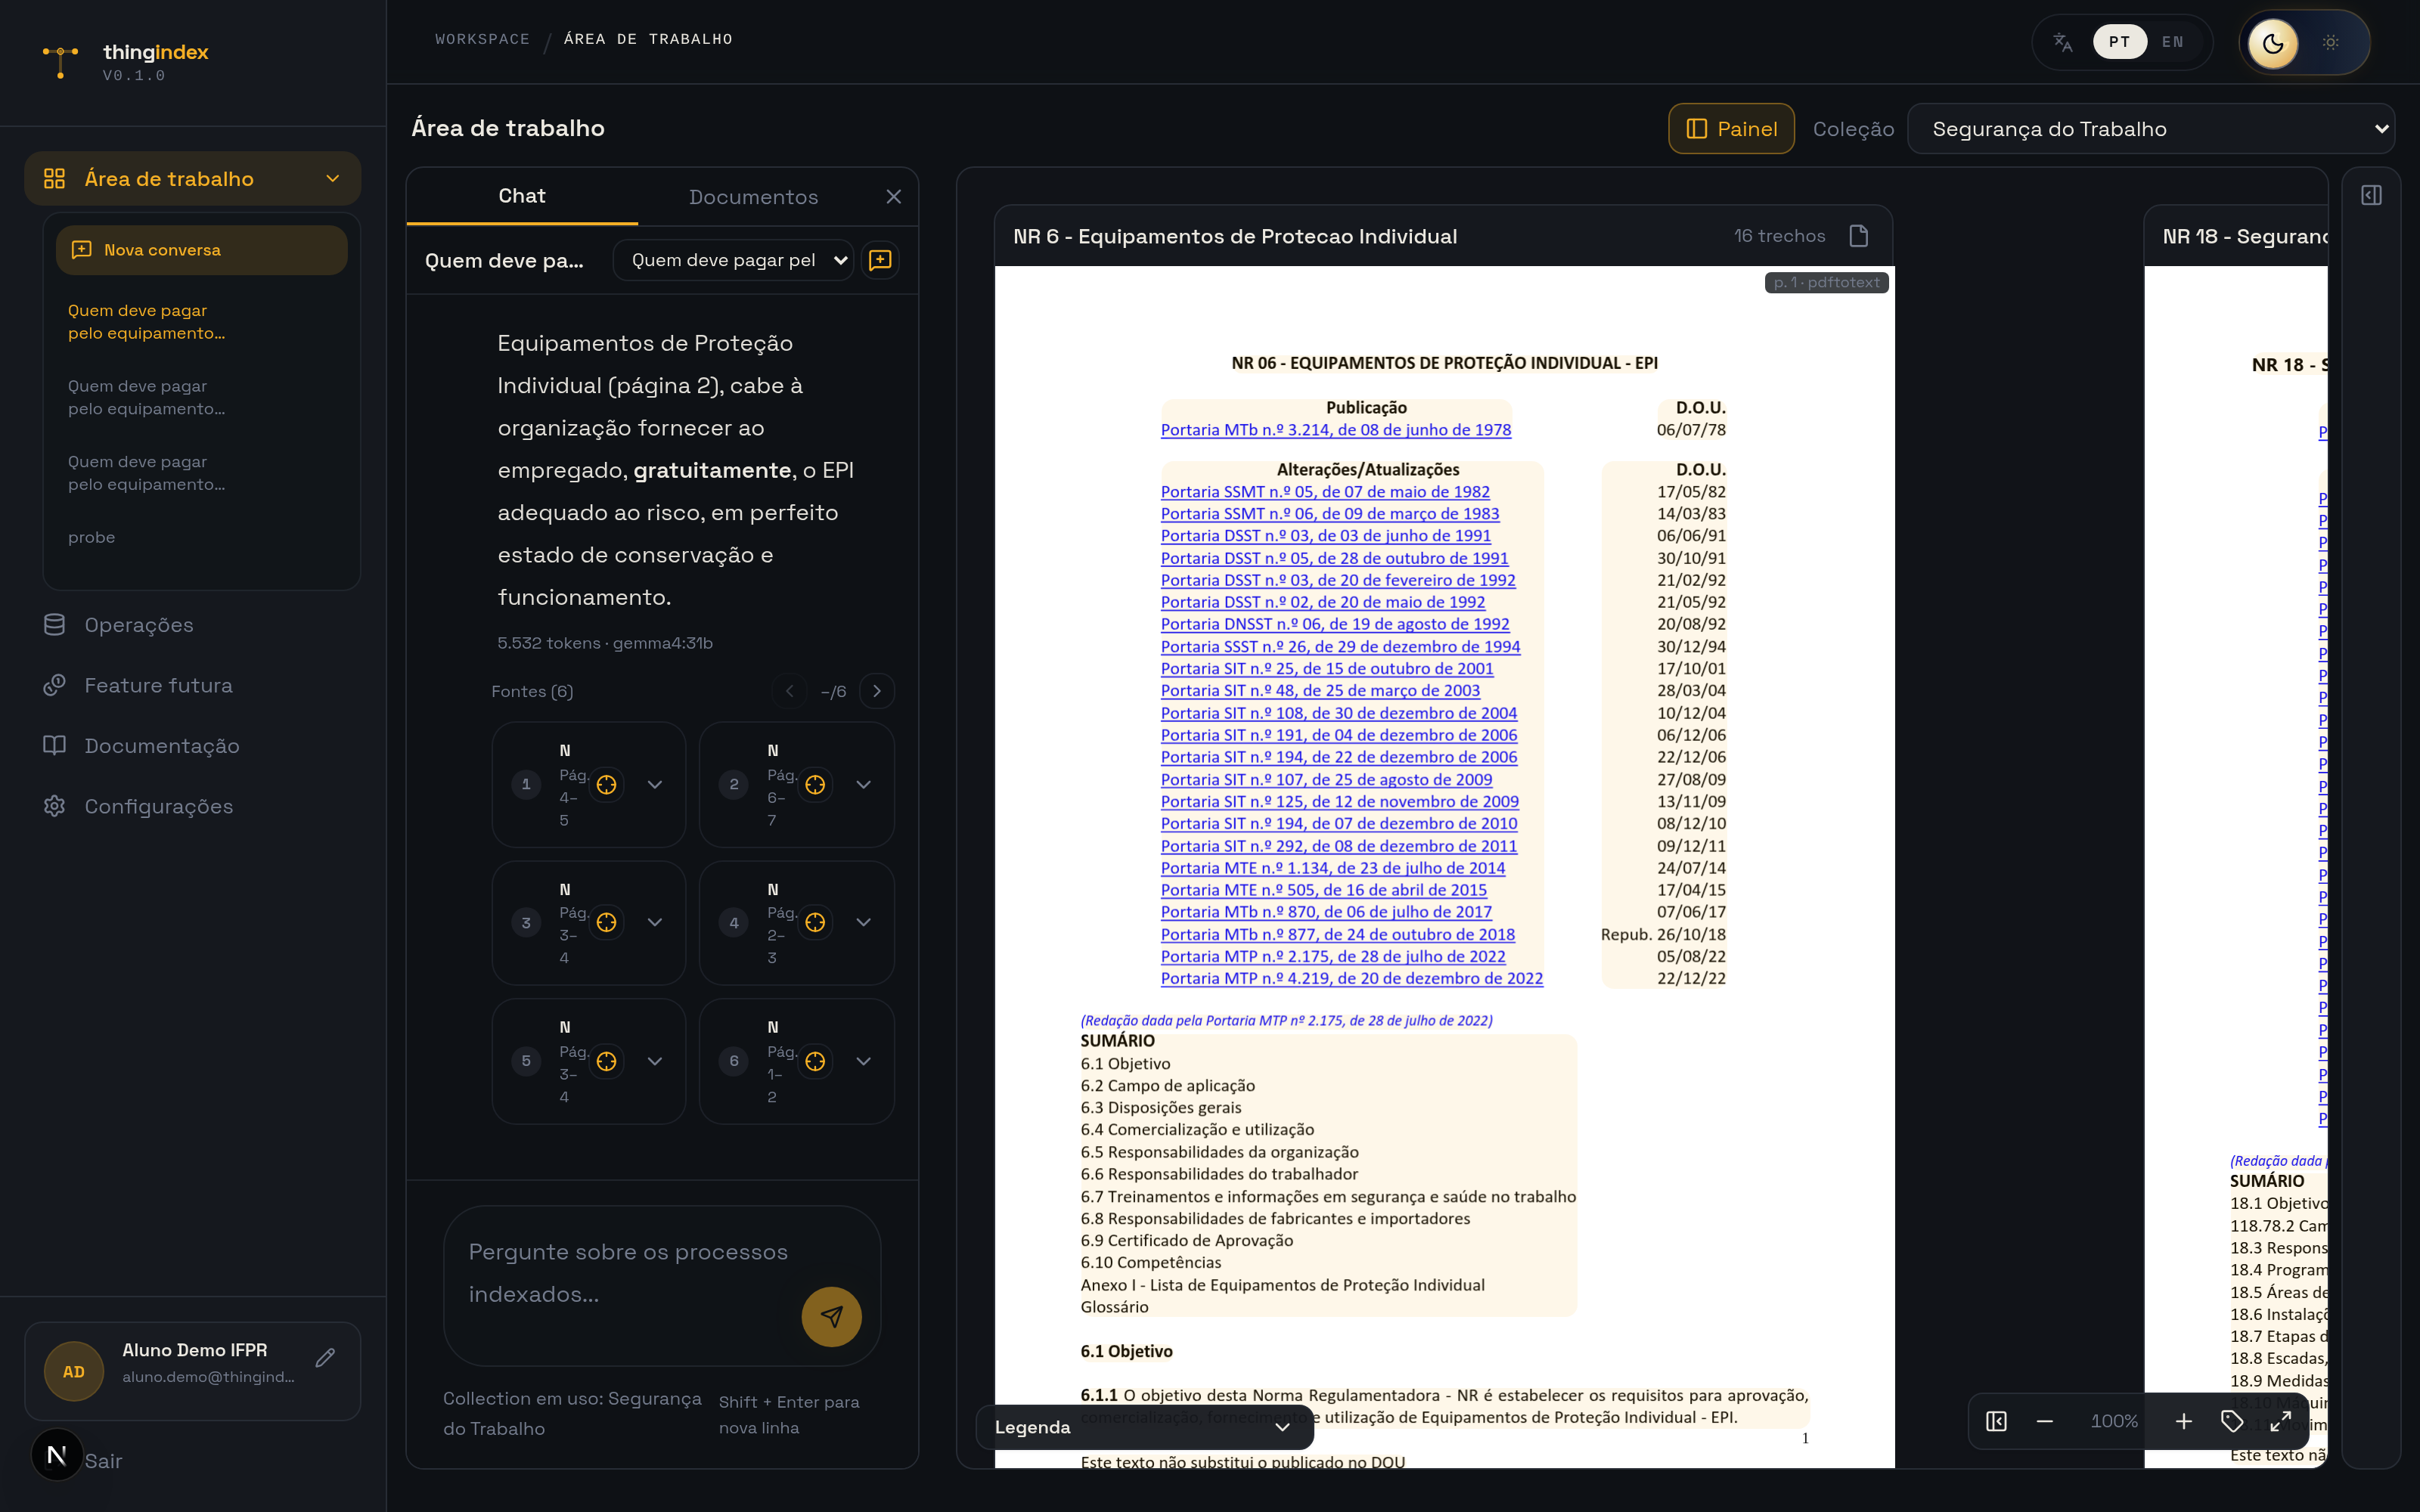
\includegraphics[width=\textwidth]{anexos/telas/workspace.png}
  \caption{\emph{Workspace} de uma coleção de normas de segurança do trabalho: \emph{chat} com a primeira fonte expandida (à esquerda), PDF na página citada com o parágrafo destacado (ao centro) e o resumo do documento gerado na indexação (à direita).}
  \label{fig:workspace}
\end{figure}

\subsection{Verificação do software}
\label{sec:verificacao}

O \emph{backend} tem \testesGoArquivos{} arquivos de teste, com \testesGoFuncoes{} funções de teste, dos quais \testesIntegracao{} são testes de integração, quase todos contra PostgreSQL, RabbitMQ ou MinIO reais; a cobertura medida foi de \coberturaBackend\% das instruções. O \emph{frontend} tem \testesFrontUnit{} arquivos de teste unitário e \testesFrontNav{} arquivos, com \testesFrontNavCasos{} casos, de teste de interface em navegador com Playwright. Há ainda um teste de caos, que derruba o RabbitMQ, o PostgreSQL e o armazenamento de arquivos com o sistema em funcionamento e confere que vinte envios simultâneos de PDF terminam indexados. As versões finais dos testes foram executadas localmente, exceto o teste de caos, que não foi executado depois da última alteração.

% =============================================================================
% 7. DESENHO DA AVALIACAO
% =============================================================================
\section{Desenho da Avaliação}
\label{sec:avaliacao}

A avaliação responde a três perguntas, nesta ordem: a busca por palavras é competitiva com a busca densa (Seções~\ref{sec:res-recuperacao} a~\ref{sec:res-determinismo})? As fontes entregues têm origem verificável (Seção~\ref{sec:res-auditabilidade})? E o sistema completo, com o modelo redigindo a resposta, acerta, cita e custa quanto (Seções~\ref{sec:res-geracao} a~\ref{sec:res-prefeitura})? A Tabela~\ref{tab:corpora} resume os acervos usados.

\begin{table}[!htbp]
\centering
\caption{Acervos e gabaritos usados na avaliação. Rep.: repetições por pergunta.}
\label{tab:corpora}
\small
\begin{tabular}{p{3.9cm}p{4.3cm}rrr}
\toprule
Acervo & Documentos & Perguntas & Rep. & Seção \\
\midrule
C1, recuperação & 5 textos sintéticos escritos pelo autor, de 111 a 166 palavras (jurídico, contratual, normativo) & 18 & -- & \ref{sec:res-recuperacao} \\
Ensino & 10 PDFs institucionais do IFPR & 72 & 3 & \ref{sec:res-geracao} \\
Legislação & Leis 8.666/1993 e 14.133/2021 & 19 & 1 & \ref{sec:res-legislacao} \\
Segurança do trabalho & 5 Normas Regulamentadoras, NR-1 em duas redações & 23 & 3 & \ref{sec:res-bateria} \\
Produto e consumidor & Código de Defesa do Consumidor, manual de monitor, termo de garantia & 23 & 3 & \ref{sec:res-bateria} \\
Licitações & Leis 8.666, 14.133 e 10.520 & 25 & 3 & \ref{sec:res-bateria} \\
Edital municipal & 1 edital de concurso, 52 páginas & 18 & 1 & \ref{sec:res-prefeitura} \\
\bottomrule
\end{tabular}
\end{table}

\textbf{Gabaritos.} Todas as perguntas foram escritas a partir dos PDFs, sem consultar o sistema. Cada uma declara o documento e a página onde está a resposta e um padrão de texto (expressão regular) que a resposta certa precisa conter; quando necessário, declara também padrões que invalidam a resposta, como os de uma recusa (``não há informação sobre isso''). Um teste automatizado confere que uma recusa genérica não conta como acerto em nenhuma pergunta que tenha resposta. Nos três acervos da bateria, cada necessidade de informação foi escrita em duas redações: uma \emph{literal}, com as palavras do documento, e uma \emph{paráfrase}, com as palavras de quem não leu o documento. O par torna mensurável um viés do próprio método: quem escreve a pergunta logo depois de ler a página tende a copiar seu vocabulário, o que favorece a busca por palavras.

\textbf{Acerto e origem.} Uma resposta é \emph{correta} quando satisfaz o gabarito; nas perguntas \emph{negativas}, que não têm resposta no acervo, quando declara que a informação não consta. A origem é medida de dois modos. A \emph{página exibida} é correta quando a página-alvo está entre as fontes mostradas pelo sistema. A \emph{página citada} é correta quando uma página escrita no texto da resposta é a página-alvo, aceitando também o número impresso no rodapé. A página citada vale para qualquer braço, inclusive para o que entrega o documento inteiro, e por isso permite comparar os dois. Nenhuma das duas confere se o trecho sustenta a frase da resposta.

\textbf{Métricas de recuperação.} Em C1, cada consulta tem documentos relevantes conhecidos, e cada braço devolve uma lista ordenada. A \emph{P@1} é a fração de consultas em que o primeiro item da lista é relevante. O \emph{MRR} dá nota 1 quando o primeiro relevante está em 1.º lugar, 1/2 quando está em 2.º, 1/3 em 3.º, e tira a média. O \emph{nDCG@10} também premia o relevante perto do topo, descontando-o pela posição entre os 10 primeiros~\cite{jarvelin2002cumulated}. As três vão de 0 a 1, e maior é melhor.

\textbf{Métricas de origem no índice.} A \emph{taxa de proveniência completa} (TPC) é a fração de unidades indexadas cuja origem está inteira no banco: documento, página, posição e conteúdo. A \emph{taxa de citação verificável} (TCV) é a fração de trechos citados que existem, letra por letra, na fonte apontada.

\textbf{Custo e modelo.} O custo é medido em \emph{tokens} enviados ao modelo por pergunta, lidos da resposta do provedor, e não em reais, porque o preço muda com o provedor e com o tempo. Todos os experimentos de geração usaram o mesmo modelo aberto, \texttt{gemma4:31b}, servido pelo Ollama em nuvem, com a temperatura padrão; nem a versão exata do modelo nem a temperatura foram fixadas, e as repetições medem a variação que resta.

\textbf{Estatística.} Na geração, a unidade de análise é a pergunta: as três repetições de uma pergunta quase sempre dão o mesmo resultado e não são observações independentes. Uma pergunta conta como acertada quando acerta nas três repetições. As tabelas trazem também a taxa por resposta, em que cada repetição conta, como descrição. Para comparar duas condições nas mesmas perguntas usou-se o teste de McNemar exato~\cite{mcnemar1947note}, que olha só as perguntas em que as condições discordam: se uma condição acerta muitas que a outra erra e quase nenhuma ao contrário, a diferença dificilmente é acaso. Os intervalos de confiança de 95\% foram obtidos por \emph{bootstrap}, sorteando as perguntas com reposição 10.000 vezes. Na recuperação, usou-se o teste de aleatorização pareado, recomendado para recuperação de informação por Smucker et al.~\citeyear{smucker2007comparison}, com a correção de Holm, que torna o teste mais exigente quando se fazem muitas comparações ao mesmo tempo.

% =============================================================================
% 8. RESULTADOS
% =============================================================================
\section{Resultados}
\label{sec:resultados}

\subsection{Busca por palavras contra busca densa}
\label{sec:res-recuperacao}

C1 é um \emph{corpus} de controle: cinco textos curtos escritos pelo autor, com 18 consultas, das quais 16 têm resposta e duas não. As consultas são de três tipos: literais (palavras tiradas do documento, o que favorece a busca por palavras), paráfrases (a mesma necessidade com outras palavras) e ruidosas (com erros de digitação e sem acentos). Seis braços foram comparados nas mesmas consultas: \textbf{A}, o pontuador anterior do sistema, que só contava ocorrências; \textbf{B}, BM25; \textbf{C}, busca densa exata com o \texttt{multilingual-e5-base}; \textbf{C$'$}, os mesmos vetores num índice aproximado IVF com $\sqrt{N}$ gavetas e uma gaveta aberta por consulta; \textbf{D}, fusão de A e B por RRF; e \textbf{E}, fusão de B e C. Mediu-se em duas unidades: o documento inteiro (5 candidatos) e a seção (19 candidatos, só nos braços lexicais, porque os vetores foram calculados por documento).

Por documento (Tabela~\ref{tab:retrieval-summary}), o BM25 e as fusões tiveram os maiores nDCG@10, de 0,890 a 0,896, seguidos da contagem (0,869), do denso exato (0,844) e do denso aproximado (0,797). A Tabela~\ref{tab:retrieval-variants} mostra de onde vêm as diferenças. Os braços lexicais acertam todas as literais e caem nas paráfrases, e a queda é maior na contagem (0,429) que no BM25 (0,286), o que se espera de um método que não dá peso à raridade das palavras. O denso quase não depende das palavras da consulta (queda de 0,029), mas acerta menos as literais (0,600). Os dois tipos de busca erram por razões diferentes, e a fusão dos dois (E) teve o maior MRR.

\begin{table}[!htbp]
\centering
\caption{Recuperação em C1 por braço, em duas unidades: documento (5 candidatos) e seção (19 candidatos; só os braços lexicais). Os intervalos de confiança de 95\% se sobrepõem em todos os braços; eles e as demais métricas estão no repositório.}
\label{tab:retrieval-summary}
\begin{tabular}{lcccccc}
\toprule
 & \multicolumn{3}{c}{Unidade: documento} & \multicolumn{3}{c}{Unidade: seção} \\
\cmidrule(lr){2-4}\cmidrule(lr){5-7}
Braço & P@1 & MRR & nDCG@10 & P@1 & MRR & nDCG@10 \\
\midrule
A, contagem     & 0,750 & 0,830 & 0,869 & 0,562 & 0,689 & 0,706 \\
B, BM25         & 0,812 & 0,861 & 0,894 & 0,750 & 0,818 & 0,829 \\
C, denso exato  & 0,688 & 0,823 & 0,844 & --    & --    & --    \\
C$'$, denso IVF & 0,688 & 0,781 & 0,797 & --    & --    & --    \\
D, RRF(A,B)     & 0,812 & 0,865 & 0,896 & 0,562 & 0,707 & 0,729 \\
E, RRF(B,C)     & 0,812 & 0,880 & 0,890 & --    & --    & --    \\
\bottomrule
\end{tabular}
\end{table}

\begin{table}[!htbp]
\centering
\caption{P@1 em C1 por tipo de consulta: literal (palavras do documento, 5 consultas), paráfrase (outras palavras, 7) e ruidosa (com erros de digitação, 4). Quanto maior a distância entre literal e paráfrase, mais o braço depende de a consulta usar as palavras do documento.}
\label{tab:retrieval-variants}
\begin{tabular}{lcccccc}
\toprule
 & \multicolumn{3}{c}{Unidade: documento} & \multicolumn{3}{c}{Unidade: seção} \\
\cmidrule(lr){2-4}\cmidrule(lr){5-7}
Braço & Literal & Paráfrase & Ruidosa & Literal & Paráfrase & Ruidosa \\
\midrule
A, contagem     & 1,000 & 0,571 & 0,750 & 1,000 & 0,143 & 0,750 \\
B, BM25         & 1,000 & 0,714 & 0,750 & 1,000 & 0,429 & 1,000 \\
C, denso exato  & 0,600 & 0,571 & 1,000 & --    & --    & --    \\
C$'$, denso IVF & 0,600 & 0,714 & 0,750 & --    & --    & --    \\
D, RRF(A,B)     & 1,000 & 0,571 & 1,000 & 1,000 & 0,143 & 0,750 \\
E, RRF(B,C)     & 0,800 & 0,714 & 1,000 & --    & --    & --    \\
\bottomrule
\end{tabular}
\end{table}

Com só 5 documentos, a medição por documento é fácil demais: um sorteio já acertaria o primeiro lugar perto de 20\% das vezes. Na unidade seção, mais próxima do que o sistema realmente devolve, as diferenças aparecem. A P@1 fica em 0,562 na contagem e 0,750 no BM25, e a revocação nos cinco primeiros (R@5) em 0,719 e 0,812. A dependência de vocabulário também cresce: na contagem, a queda da literal para a paráfrase passa de 0,429 por documento para 0,857 por seção, e o pontuador acerta só 14\% das paráfrases. Esse resultado motivou a troca da contagem pelo BM25, que é o pontuador de todos os experimentos seguintes.

Nenhuma das 75 comparações entre pares de braços foi estatisticamente significativa depois da correção de Holm (o menor valor-$p$ sem correção foi 0,125). Isso decorre do tamanho do teste: com 16 consultas, no máximo 8 diferem em qualquer comparação, o que é pouco para detectar diferenças dessa ordem. A diferença de P@1 entre BM25 e denso exato foi de $+0{,}125$, com intervalo de 95\% de $-0{,}188$ a $+0{,}438$. C1, portanto, não mostra que a busca por palavras seja igual ou melhor que a densa; mostra apenas que, neste \emph{corpus}, nenhuma diferença foi detectável.

\subsection{Quando não há resposta}
\label{sec:res-ausencia}

Nas duas consultas de C1 sem resposta, todos os braços devolveram resultados. Na busca por palavras, qualquer palavra em comum já gera nota positiva. Na densa, a similaridade entre pergunta e texto relevante (de 0,785 a 0,881) e entre pergunta e texto irrelevante (de 0,763 a 0,848) quase se sobrepõe, o que os autores do E5 já indicam ao recomendar usar a ordem dos resultados, e não o valor da nota~\cite{e5modelcard2023}. Nos dois tipos de busca, a nota não serve para decidir que não há resposta. O sistema completo, porém, se comporta de outro modo: instruído a responder só a partir das fontes, o modelo declarou que a informação não consta em todas as perguntas negativas medidas, as 5 do acervo de ensino e as 9 da bateria, nas três repetições. A ausência é reconhecida na redação da resposta, e não na busca.

\subsection{Estabilidade dos resultados}
\label{sec:res-determinismo}

Um requisito do sistema é que a mesma pergunta traga sempre as mesmas fontes. Cada braço de C1 foi executado 30 vezes, e as listas completas foram comparadas por \emph{hash}. Contagem, BM25, a fusão dos dois e a busca densa exata deram listas idênticas em todas as execuções. A variação, portanto, não vem do modelo de vetores. No índice aproximado C$'$, mudar a semente aleatória que forma as gavetas ou a ordem de inserção dos documentos produziu até quatro listas diferentes para a mesma consulta, com perda média de 48,4\% da revocação da busca exata.

Essa configuração, porém, não é a que o pgvector recomenda. Para saber se a instabilidade é do índice aproximado em si ou da configuração, as opções foram medidas no próprio pgvector, com 1.000 a 20.000 vetores sintéticos (Tabela~\ref{tab:ann-pgvector}). Cada índice foi reconstruído cinco vezes sobre os mesmos dados e depois construído com os vetores inseridos em cinco ordens diferentes.

% GERADO POR scripts/ann-pgvector.py a partir de docs/article/results/ann-pgvector.csv -- nao edite a mao.
\begin{table}[htb]
\centering
\caption{Índices aproximados do pgvector 0.8.6 sobre corpora sintéticos (768 dimensões, 20 consultas). Revocação@10 frente à busca exata e número de consultas cujo top-10 mudou ao reconstruir o índice 5 vezes sobre os mesmos dados e ao inserir os mesmos vetores em 5 ordens.}
\label{tab:ann-pgvector}
\small
\begin{tabular}{lrrrr}
\hline
Índice & $N$ & Revocação@10 & Reconstrução & Ordem \\
\hline
IVFFlat, $\sqrt{N}$ listas, 1 sonda & 1.000 & 47{,}7\% & 20/20 & 20/20 \\
IVFFlat, recomendação do pgvector & 1.000 & 100{,}0\% & 0/20 & 0/20 \\
HNSW, padrões do pgvector & 1.000 & 100{,}0\% & 0/20 & 0/20 \\
\hline
IVFFlat, $\sqrt{N}$ listas, 1 sonda & 5.000 & 36{,}5\% & 20/20 & 20/20 \\
IVFFlat, recomendação do pgvector & 5.000 & 100{,}0\% & 0/20 & 0/20 \\
HNSW, padrões do pgvector & 5.000 & 99{,}0\% & 2/20 & 4/20 \\
\hline
IVFFlat, $\sqrt{N}$ listas, 1 sonda & 20.000 & 25{,}5\% & 20/20 & 20/20 \\
IVFFlat, recomendação do pgvector & 20.000 & 100{,}0\% & 0/20 & 0/20 \\
HNSW, padrões do pgvector & 20.000 & 91{,}0\% & 6/20 & 17/20 \\
\hline
\end{tabular}
\end{table}


Com a configuração recomendada, o IVFFlat deu sempre o mesmo resultado da busca exata, porque nessas escalas ela usa poucas gavetas e abre boa parte delas. A configuração de $\sqrt{N}$ gavetas e uma só aberta perdeu mais da metade da revocação e mudou o resultado de todas as consultas, até ao reconstruir o índice sobre os mesmos dados. O HNSW com os parâmetros padrão foi exato e estável com 1.000 vetores; com 20.000, a revocação caiu para 91,0\%, e 6 das 20 consultas mudaram ao reconstruir o índice e 17 ao mudar a ordem de inserção (conta como mudança qualquer troca entre os 10 primeiros, e a tabela é uma única execução). A instabilidade depende da configuração e da escala, e não é inevitável: nas coleções que o ThingIndex atende, de até alguns milhares de unidades, um índice vetorial bem configurado também seria estável. A estabilidade, portanto, não é uma vantagem exclusiva da busca por palavras.

\subsection{Origem das fontes no índice}
\label{sec:res-auditabilidade}

Na versão atual, as 155 unidades indexadas de C1 têm TPC de 1,000 em todos os tipos de estrutura. A primeira medição, porém, deu 0,329: 104 unidades estavam incompletas, todas por falta de página. Dezenove eram um defeito de modelagem: a tabela de trechos não tinha coluna de página, e como o trecho é o que se cita como fonte, a coordenada precisava estar nele. A coluna foi criada e é preenchida com a página do primeiro parágrafo do trecho. As outras 85 não eram defeito: eram estatísticas do documento inteiro, como o número de parágrafos, que não estão em página nenhuma. Em vez de contá-las como falha ou dar a elas uma página inventada, cada unidade passou a declarar se sua origem é uma página ou o documento inteiro. A Tabela~\ref{tab:provenance-evolucao} separa os dois efeitos, porque o valor final sozinho não distinguiria uma correção real de um ajuste da métrica.

\begin{table}[!htbp]
\centering
\caption{Evolução da TPC sobre C1 (155 unidades).}
\label{tab:provenance-evolucao}
\begin{tabular}{lccc}
\toprule
 & Critério original & + página no trecho & + escopo de origem \\
\midrule
Unidades completas & 51 & 70 & 155 \\
TPC & 0,329 & 0,452 & 1,000 \\
\bottomrule
\end{tabular}
\end{table}

Duas ressalvas limitam esse 1,000. C1 é texto sem paginação, e nele toda unidade fica na página 1; a TPC mostra que o mecanismo carrega a coordenada, e não que ela esteja certa. A página certa é conferida por testes unitários com parágrafos em páginas diferentes e, nos PDFs reais, pela página exibida nas seções seguintes. Além disso, a TPC mede o índice, e não a resposta. A TCV foi de 1,000 sobre 20 citações de C1: todo trecho citado existe no documento apontado. Por fim, a TPC depende de como se guarda, e não de como se busca: uma coluna de vetores na mesma tabela, com a mesma chave estrangeira, teria a mesma TPC.

\subsection{Trechos recuperados contra documento inteiro}
\label{sec:res-geracao}

Este experimento mede o sistema como o usuário o encontra e o compara com a alternativa de entregar o documento inteiro ao modelo. No braço \textbf{T}, o avaliador usa a mesma rota de \emph{chat} que a tela usa. No braço \textbf{F}, o mesmo modelo recebe o texto completo do documento que contém a resposta, com o número de cada página marcado, sem nenhuma busca; nas perguntas negativas, recebe cinco documentos. F é um teto otimista, porque já sabe qual é o documento certo, informação que um usuário não teria. O acervo de ensino tem 10 PDFs e 72 perguntas, de quatro tipos: prosa, tabela, calendário e negativa.

Este é o acervo de desenvolvimento, e o resultado deve ser lido assim: o braço T foi ajustado várias vezes contra essas 72 perguntas, passando de 67 de 72 a 216 de 216 respostas certas, e o gabarito passou por quatro versões no mesmo período. O braço F foi executado uma vez, sem ajuste. Doze perguntas tinham sido usadas diretamente para calibrar o sistema, e os resultados sem elas são dados à parte.

\textbf{Acerto.} Por pergunta, T acertou as 72 e F, 71: F errou a mesma negativa nas três repetições (Tabela~\ref{tab:geracao}). Sem as 12 perguntas de calibração, os números são 60 de 60 e 59 de 60. A diferença é de uma pergunta e no acervo em que T foi ajustado: o experimento mostra que buscar antes de perguntar não custou acerto aqui, mas não autoriza afirmar que os dois se equivalem em outros acervos.

\begin{table}[!htbp]
\centering
\caption{Geração no acervo de ensino (desenvolvimento), 72 perguntas, três repetições: acerto por resposta, página exibida (só existe em T), página citada no texto e \emph{tokens} enviados ao modelo por pergunta. As colunas de página contam as 201 respostas que têm página-alvo.}
\label{tab:geracao}
\small
\begin{tabular}{lrrrrrrr}
\toprule
 & \multicolumn{2}{c}{Acerto} & Pág. exibida & \multicolumn{2}{c}{Pág. citada} & \multicolumn{2}{c}{\emph{Tokens}/pergunta} \\
Tipo & T & F & T & T & F & T & F \\
\midrule
Prosa (30)      & 1,000 & 1,000 & 0,933 & 0,933 & 0,889 & 3.629 & 100.491 \\
Tabela (21)     & 1,000 & 1,000 & 1,000 & 0,905 & 0,968 & 3.619 & 39.691 \\
Calendário (16) & 1,000 & 1,000 & 1,000 & 1,000 & 1,000 & 6.400 & 5.504 \\
Negativa (5)    & 1,000 & 0,800 & -- & -- & -- & 3.241 & 250.504 \\
\midrule
Todas (72)      & 1,000 & 0,986 & 0,970 & 0,940 & 0,940 & 4.215 & 72.067 \\
\bottomrule
\end{tabular}
\end{table}

\textbf{Custo.} Em média, T enviou 4.215 \emph{tokens} por pergunta e F, 72.067. Sem as negativas, em que F recebe cinco documentos, as médias são 4.288 e 58.751, 13,7 vezes mais em F. Pergunta a pergunta, F usou de 0,7 a 96 vezes os \emph{tokens} de T, com mediana de 26,5 (o 1/26 do resumo). T gastou mais que F em 22 das 72 perguntas, todas sobre documentos curtos, em que várias páginas recuperadas somam mais que o documento inteiro. O custo de T depende do número de fontes, e o de F cresce com o documento: numa execução exploratória com outro modelo, de janela de 131 mil \emph{tokens}, a entrega da coleção inteira foi recusada pelo provedor por exceder esse limite (227.649 \emph{tokens}).

\textbf{Origem.} A página citada no texto esteve correta em 189 de 201 respostas em T e em 189 de 201 em F, 0,940 nos dois; sem aceitar o número impresso no rodapé da página, F cairia para 173. O que muda é de onde vem a página. Em F, a página só existe no texto escrito pelo modelo, e na pergunta que F errou a resposta afirma um dado inexistente e o atribui a uma página do documento. Em T, a página mostrada na fonte vem do banco e não pode ser inventada; a página-alvo esteve entre as fontes exibidas em 195 de 201 respostas. O modelo, porém, também escreve páginas no texto em T, e essas podem estar erradas.

Com acerto de 1,000, este acervo deixou de distinguir boas e más versões do sistema, em parte porque o sistema foi ajustado nele. Os acervos seguintes têm perguntas escritas depois do desenvolvimento.

\subsection{Legislação com norma revogada}
\label{sec:res-legislacao}

O acervo de legislação tem duas leis: a 8.666/1993 e a 14.133/2021, que a revogou. Conforme a data e o contrato, a mesma pergunta pode ter respostas diferentes, e os dois textos usam quase o mesmo vocabulário, o que é difícil para qualquer busca por semelhança. É o conflito entre fontes descrito por Xu et al.~\citeyear{xu2024knowledge}. Das 19 perguntas, as \emph{divergentes} exigem distinguir as duas leis, e responder só pela revogada conta como erro.

O sistema acertou 15 das 19 perguntas (0,789; Tabela~\ref{tab:dominio2}). Uma das quatro respostas erradas é erro do gabarito, que exigia ``10 (dez) anos'' quando a resposta dizia ``10 anos''; o gabarito não foi alterado depois de medir, e o acerto real é 16 de 19. A falha que motivou este acervo apareceu nas divergentes: perguntado se a modalidade ``tomada de preços'' existe, o sistema respondeu que sim e citou corretamente o art.~22 da Lei 8.666, sem dizer que ele foi revogado. A citação e a página estão certas, e a resposta é enganosa: quem conferir a fonte vai confirmar um dispositivo que já não vale. O mesmo aconteceu com o limite de dispensa de licitação para obras. Com uma repetição e 19 perguntas, o resultado é descritivo.

\begin{table}[!htbp]
\centering
\caption{Acervo de legislação: 19 perguntas, uma repetição. Pág. exibida: a página-alvo está entre as fontes mostradas, nas 16 perguntas que têm página-alvo.}
\label{tab:dominio2}
\begin{tabular}{lrrrr}
\toprule
Tipo & $n$ & Acerto & Pág. exibida & \emph{Tokens}/pergunta \\
\midrule
Divergente & 5 & 0,600 & 0,800 & 5.406 \\
Temporal   & 3 & 1,000 & 1,000 & 7.147 \\
Prosa      & 8 & 0,750 & 0,750 & 6.204 \\
Negativa   & 3 & 1,000 & --    & 5.588 \\
\midrule
Total      & 19 & 0,789 & 0,812 & 6.045 \\
\bottomrule
\end{tabular}
\end{table}

\subsection{Bateria em três domínios}
\label{sec:res-bateria}

A bateria mede o sistema em três acervos de áreas diferentes (segurança do trabalho, produto e consumidor, licitações), com perguntas escritas depois do desenvolvimento. O acervo de licitações repete as duas leis do anterior e acrescenta a Lei 10.520, de modo que os dois não são independentes. As perguntas têm cinco formas: \emph{aberta} (pede um dado), \emph{confirmação} (sim ou não), \emph{existência} (o acervo trata do assunto?), \emph{premissa falsa} (a pergunta traz um dado errado, e a resposta certa é corrigi-lo) e \emph{negativa}. São 71 perguntas, 31 delas em pares literal e paráfrase, com três repetições, num total de 213 respostas.

Com a pergunta original, a taxa de acerto foi de 0,695, com os três acervos entre 0,623 e 0,826 e intervalos que se sobrepõem (Tabela~\ref{tab:bateria-tema}). Por pergunta, 49 das 71 acertaram nas três repetições, 21 erraram nas três e só 1 oscilou: os erros se repetem entre execuções. A página-alvo esteve entre as fontes exibidas em 58,1\% das respostas, abaixo do acerto, porque uma resposta certa pode vir de outra página com a mesma informação, o que é comum em acervos com documentos sobrepostos.

\begin{table}[!htbp]
\centering
\caption{Bateria, pergunta original: acerto por acervo. Por resposta, com intervalo de 95\% por \emph{bootstrap} (sorteando perguntas), e por pergunta (acerto nas três repetições).}
\label{tab:bateria-tema}
\begin{tabular}{lrrrr}
\toprule
Acervo & Respostas & Acerto & Intervalo 95\% & Perguntas \\
\midrule
Segurança do trabalho & 69 & 0,623 & 0,435--0,812 & 14/23 \\
Produto e consumidor  & 69 & 0,826 & 0,652--0,957 & 19/23 \\
Licitações            & 75 & 0,640 & 0,440--0,840 & 16/25 \\
\midrule
Total                 & 213 & 0,695 & 0,592--0,793 & 49/71 \\
\bottomrule
\end{tabular}
\end{table}

Esses números usam o gabarito revisado depois da primeira medição. A versão original aceitava um ``não'' ou um ``há'' isolados em duas formas de pergunta, e uma resposta fixa de recusa (``Não há informações sobre isso nos documentos fornecidos'') acertaria 24 perguntas. A revisão passou a exigir, na premissa falsa, o dado que a corrige, e a invalidar recusas e respostas opostas onde elas não são a resposta certa. Todas as respostas cujo veredito mudou foram conferidas à mão, e o acerto caiu de 0,817 para 0,695. Na forma existência, cuja resposta certa é sempre ``sim'', responder ``Sim.'' a tudo acertaria as 12 perguntas, de modo que o 0,917 dessa forma só mostra que o sistema não negou um assunto presente.

Por forma (Tabela~\ref{tab:bateria-forma}), o sistema reconheceu a falta de informação em todas as negativas, e as perguntas que pedem um dado ficaram entre 0,61 e 0,75. A premissa falsa foi a mais difícil: em só 13 de 36 respostas o sistema corrigiu o dado errado. Nas demais, disse que o acervo não trazia a informação ou respondeu dentro da premissa, como na pergunta sobre como abrir uma licitação na modalidade ``tomada de preços'', em que ensinou o procedimento da lei revogada. É a bajulação descrita por Sharma et al.~\citeyear{sharma2024sycophancy}, somada ao problema de vigência da seção anterior.

\begin{table}[!htbp]
\centering
\caption{Bateria, pergunta original: acerto por forma da pergunta, nos três acervos (respostas).}
\label{tab:bateria-forma}
\begin{tabular}{lrr}
\toprule
Forma & Acertos & Taxa \\
\midrule
Negativa       & 27/27 & 1,000 \\
Existência     & 33/36 & 0,917 \\
Confirmação    & 27/36 & 0,750 \\
Aberta         & 48/78 & 0,615 \\
Premissa falsa & 13/36 & 0,361 \\
\bottomrule
\end{tabular}
\end{table}

\textbf{Redação da pergunta.} Por resposta, o acerto foi 0,882 nas literais e 0,419 nas paráfrases. Como as duas versões de um par pedem a mesma coisa, a comparação é feita por par. Dos 31 pares, 17 foram concordantes (mesmo resultado nas duas versões) e 14 discordantes, todos a favor da literal: a literal acertou e a paráfrase errou, sem nenhum caso contrário ($p < 0{,}001$ no teste de McNemar). A direção foi a mesma nos três acervos (7, 4 e 3 pares). Esse resultado depende da revisão do gabarito: com a versão original, eram 8 pares a favor da literal e 2 a favor da paráfrase ($p = 0{,}109$). O sistema acerta muito melhor quando a pergunta usa as palavras do documento, que é exatamente o ponto fraco da busca por palavras descrito na Seção~\ref{sec:ref-ri}.

\subsection{Primeira tentativa: enriquecer o índice}
\label{sec:res-enriquecimento}

Se o usuário não usa as palavras do documento, uma saída é acrescentar ao índice as palavras que ele usaria. A primeira intervenção fez isso: para cada página, o LLM gerou um resumo e perguntas que a página responde, escritas como um leigo as escreveria. O pré-registro previa três braços (só o conteúdo, conteúdo mais resumo, conteúdo mais perguntas geradas), 16 pares de perguntas e os três acervos da bateria. A execução, porém, usou 12 perguntas, 5 delas em pares, de um só acervo, o de segurança do trabalho, e acrescentou um quarto braço exploratório. Pelo desvio em relação ao pré-registro, o resultado é exploratório.

Uma primeira execução foi descartada: uma auditoria mostrou fontes idênticas nos quatro braços, o que é impossível se cada braço busca em textos diferentes. A troca de braço, feita por variável de ambiente, não tinha chegado ao processo que respondia. O experimento foi refeito com um processo da API por braço, e o pré-registro recebeu um adendo.

Na reexecução (Tabela~\ref{tab:enriquecimento}), as fontes mudaram entre os braços em 8 das 12 perguntas, mas o acerto quase não mudou, e as quatro paráfrases que erravam continuaram erradas em todos os braços. Com 5 paráfrases e uma repetição, o experimento não teria como detectar um efeito moderado, e o resultado é a ausência de efeito detectável. Lendo as perguntas geradas, a explicação mais provável é que o modelo, mesmo instruído a escrever como leigo, repete o vocabulário do documento. Há muitas formas de pedir a mesma coisa, e o índice recebe uma delas, raramente a que o usuário vai usar. Isso é compatível com Gospodinov et al.~\citeyear{gospodinov2023doc2query}, que mostraram que parte do texto gerado para expandir documentos é ruído.

\begin{table}[!htbp]
\centering
\caption{Enriquecimento do índice: 12 perguntas de segurança do trabalho, uma repetição por braço (reexecução, gabarito revisado). Pág. exibida: nas 10 perguntas que têm página-alvo.}
\label{tab:enriquecimento}
\begin{tabular}{lrrrr}
\toprule
Braço & Geral & Literal & Paráfrase & Pág. exibida \\
\midrule
Só conteúdo               & 7/12 & 4/5 & 1/5 & 5/10 \\
Conteúdo + resumo         & 8/12 & 5/5 & 1/5 & 5/10 \\
Conteúdo + perguntas      & 7/12 & 4/5 & 1/5 & 5/10 \\
Máximo (exploratório)     & 8/12 & 5/5 & 1/5 & 5/10 \\
\bottomrule
\end{tabular}
\end{table}

\subsection{Segunda tentativa: expandir a pergunta}
\label{sec:res-expansao}

A segunda intervenção vai no sentido contrário: em vez de levar as palavras do leigo ao documento, leva as palavras do documento à pergunta, como em Jagerman et al.~\citeyear{jagerman2023qe}. Ir de muitas formulações para o termo técnico que nomeia a necessidade é mais fácil que o contrário. A hipótese pré-registrada foi que a expansão melhoraria as paráfrases e deixaria as literais quase iguais.

O modelo recebe só o texto da pergunta e devolve termos técnicos relacionados, que são acrescentados à busca. Ele não vê o acervo nem o gabarito, e as 71 perguntas são as mesmas da bateria. O modelo que expande é o mesmo que depois responde. Para a pergunta ``Quem paga o capacete e a luva que eu uso no serviço?'', que errava nas três repetições, a expansão gerou \emph{equipamento, proteção, individual, EPI, fornecedor, empregador, custo, pagamento}, e a resposta passou a citar a página certa da NR-6.

Com a expansão, a distância entre literal e paráfrase cai de 0,462 para 0,065 (Tabela~\ref{tab:expansao}). Nas mesmas 71 perguntas, 14 passaram a acertar nas três repetições e nenhuma deixou de acertar ($p < 0{,}001$ no teste de McNemar). A diferença foi de 0,197, com intervalo de 95\% de 0,105 a 0,290; por resposta, o acerto com expansão tem intervalo de 0,803 a 0,958, contra 0,592 a 0,793 sem ela. O resultado não depende da revisão do gabarito: com o gabarito original, o efeito já era significativo (10 ganhos e 1 perda, $p = 0{,}012$). Das perguntas que erravam sem expansão, a expansão corrigiu 13 de 18 paráfrases e 1 de 4 literais, na direção prevista, e a página-alvo passou a ser exibida em 0,823 das respostas, contra 0,581. Os \emph{tokens} enviados para responder cresceram 13,4\%, e cada pergunta nova exige uma chamada a mais ao modelo.

\begin{table}[!htbp]
\centering
\caption{Expansão da pergunta: pergunta original contra pergunta expandida, nas 71 perguntas da bateria. Acerto e página exibida por resposta (213 por condição); a última coluna é o acerto por pergunta, nas três repetições.}
\label{tab:expansao}
\small
\begin{tabular}{lrrrrrr}
\toprule
Condição & Literal & Paráfrase & Todas & Pág. exibida & \emph{Tokens}/pergunta & Perguntas \\
\midrule
Sem expansão & 0,882 & 0,419 & 0,695 & 0,581 & 4.699 & 49/71 \\
Com expansão & 0,903 & 0,839 & 0,887 & 0,823 & 5.327 & 63/71 \\
\bottomrule
\end{tabular}
\end{table}

Três cuidados limitam esse ganho. O controle é a execução anterior da bateria, feita no mesmo dia, e não um braço sorteado junto. Os três acervos são documentos públicos, que o modelo provavelmente viu no treinamento: ``empregador'', gerado para a pergunta sobre quem paga o equipamento, é ao mesmo tempo uma ponte de vocabulário e a própria resposta, e o ganho não pode ser estendido a documentos internos de uma organização. E não houve comparação com expansão sem LLM nem com busca híbrida. Como a primeira ocorrência de cada pergunta depende do modelo, a expansão ficou desligada por padrão; a partir da segunda, o resultado sai de um \emph{cache} e a busca volta a ser determinística.

\subsection{Edital municipal (exploratório)}
\label{sec:res-prefeitura}

Por fim, o sistema foi aplicado ao edital de um concurso público municipal, com 52 páginas, tabelas de cargos que atravessam páginas e dois capítulos com o mesmo número por erro do próprio edital. As 18 perguntas, em nove pares, foram escritas para provocar um tipo de falha cada. O sistema acertou 15 de 18. As duas versões da pergunta que pede o total de vagas somando uma tabela de três páginas erraram, porque a busca trouxe só parte das páginas e o modelo somou o que viu. A terceira falha foi de busca: a pergunta pelo ``Capítulo XVI'' não trouxe a página do capítulo, porque o numeral romano pesa pouco no BM25. Somar linhas espalhadas por muitas páginas é um limite concreto de uma busca com número fixo de fontes. Com um documento e uma repetição, o resultado é descritivo.

% =============================================================================
% 9. DISCUSSAO
% =============================================================================
\section{Discussão}
\label{sec:discussao}

\textbf{Resposta à pergunta de pesquisa.} Nos acervos medidos, unidades de PDF guardadas em tabelas relacionais e buscadas por BM25 sustentaram um sistema cujas fontes podem ser conferidas: a coordenada de cada fonte vem do banco, o esquema a exige e um teste confere isso. Nos acervos com perguntas escritas depois do desenvolvimento, a taxa de acerto foi de 0,695 com a pergunta original e de 0,887 com a expansão. A resposta à pergunta de pesquisa é afirmativa nessa escala, de três a cinco documentos por acervo de teste e perguntas em português, com duas ressalvas: o acerto depende muito de como a pergunta é escrita, e uma fonte verificável não garante uma resposta atual.

\textbf{O que a garantia de origem cobre.} Com o documento inteiro, o modelo citou a página certa tantas vezes quanto com a busca (0,940). A diferença é que, com a busca, o leitor recebe uma página que vem do banco e não pode ter sido inventada pelo modelo. Essa garantia vem de guardar as unidades com coordenada, e não do BM25: uma coluna de vetores na mesma tabela daria a mesma garantia. Como a busca por palavras não teve diferença detectável da densa em C1 e um índice vetorial bem configurado foi estável na escala do ThingIndex, dispensar o banco vetorial fica como uma escolha de simplicidade de operação, e não como uma vantagem de qualidade demonstrada. Os dados de C1, em que os dois tipos de busca erram por razões diferentes, indicam a busca híbrida dentro do próprio PostgreSQL como o próximo passo.

\textbf{Limitações medidas.} A redação teve o maior efeito: as paráfrases acertaram 0,419 contra 0,882 das literais. A expansão reduziu essa distância a 0,065, mas foi medida só com documentos públicos e continua desligada por padrão. A vigência foi o erro mais grave: o sistema trata como independentes documentos que se revogam e responde com fonte correta e conteúdo desatualizado. Como a conferência da fonte confirma o erro, o sistema, na versão atual, não é adequado para acervos com normas revogadas, a menos que a coleção contenha só as versões vigentes. Por fim, respostas que exigem somar linhas de muitas páginas ficam limitadas pelo número de fontes.

\textbf{Sobre o método.} Os controles se mostraram necessários. O acervo de desenvolvimento chegou a 1,000, número que não se repetiu em nenhum acervo de teste. A primeira execução do enriquecimento deu um resultado nulo que parecia sólido, mas não tinha medido o que dizia medir, e o problema só apareceu ao comparar as fontes. E a revisão do gabarito da bateria mostrou que recusas e até respostas opostas eram aceitas como acerto, o que inflava o resultado em 0,122. Nos três casos, a correção só foi possível porque os dados brutos estavam guardados pergunta a pergunta.

\subsection{Ameaças à validade}
\label{sec:ameacas}

\textbf{Amostras pequenas.} C1 tem 16 consultas com resposta, pouco para qualquer comparação de recuperação ser significativa. A bateria tem 71 perguntas, e as duas versões de um par não são independentes. Os acervos de legislação e do edital têm uma repetição.

\textbf{Um único autor.} O sistema foi ajustado no acervo de ensino. Todos os gabaritos foram escritos pelo autor, sem segunda anotação nem medida de concordância como o $\kappa$ de Cohen~\citeyear{cohen1960coefficient}, e as paráfrases foram escritas por quem já tinha lido o documento. O critério por expressão regular pode aceitar resposta incompleta e recusar resposta certa redigida de outro modo; os dois casos foram encontrados e corrigidos onde vistos.

\textbf{O que se mediu.} A página exibida e a página citada não medem se o trecho sustenta a frase da resposta. A página-alvo subestima o acerto da citação quando a informação está em mais de uma página.

\textbf{Generalização.} Todos os documentos estão em português, e o maior acervo tem 10 PDFs. Um único modelo redigiu as respostas, sem versão nem temperatura fixadas; uma medição exploratória com outro modelo, maior, só no braço F, deu acerto de 0,742 contra 1,000 do modelo principal nas mesmas 66 perguntas, descontadas 6 falhas da API do provedor, o que indica que os números dependem do modelo. Os acervos de teste são públicos, e não se mediu o comportamento com documentos internos. A utilidade para usuários reais não foi avaliada.

% =============================================================================
% 10. CONCLUSAO
% =============================================================================
\section{Conclusão}
\label{sec:conclusao}

Este trabalho apresentou o ThingIndex, um sistema que guarda a estrutura dos PDFs em tabelas relacionais e responde perguntas mostrando documento, página e região de cada fonte. O sistema foi implementado, testado inclusive sob falha da infraestrutura, e avaliado em sete acervos. Os principais resultados são três. Primeiro, a origem de cada fonte vem do banco e é exigida pelo esquema, e só a busca oferece ao leitor uma página que não foi escrita pelo modelo. Segundo, com perguntas escritas depois do desenvolvimento, a taxa de acerto foi de 0,695 com a pergunta original. As paráfrases acertaram bem menos que as literais, e a expansão da pergunta elevou o acerto a 0,887, em configuração experimental e medida só em documentos públicos. Terceiro, buscar trechos usou, na mediana, 1/26 dos \emph{tokens} de entregar o documento inteiro, sem perda de acerto no acervo de desenvolvimento. Não houve diferença detectável entre a busca por palavras e a densa, e dispensar o banco vetorial é uma escolha de simplicidade.

A limitação mais séria é a vigência: o sistema cita corretamente uma norma revogada, e conferir a fonte não revela o erro. O modelo relacional oferece um caminho, com datas de vigência por unidade do documento e comparação de períodos em SQL, como no padrão temporal do SQL:2011~\cite{kulkarni2012temporal}; a vigência precisa ser registrada por artigo, e não só por documento, porque a revogação pode ser parcial.

Os trabalhos futuros, em ordem de prioridade, são: tratar a vigência por unidade do documento; avaliar o sistema com usuários reais, medindo o tempo até a resposta e se as fontes são de fato conferidas; medir se o trecho exibido sustenta a frase da resposta; ampliar os gabaritos, com um segundo anotador e documentos que o modelo não conhece; e comparar a expansão e a busca híbrida no próprio PostgreSQL.

O código, os gabaritos, os resultados brutos, os diagramas e os \emph{scripts} que geram e conferem os números deste artigo estão no repositório do projeto, \repositorio.

\subsection*{Declaração sobre o uso de inteligência artificial generativa}

Foram usados assistentes de IA generativa (ChatGPT, da OpenAI, e Claude, da Anthropic) como apoio à revisão de erros ortográficos e a uma leitura crítica simulada do trabalho antes da entrega. Essa leitura crítica levou a correções relatadas no texto, como a revisão do gabarito da bateria e a medição dos índices no próprio pgvector. A escrita do artigo, o desenho da pesquisa, as hipóteses, os gabaritos, o desenvolvimento e as decisões técnicas são do autor. Todo o conteúdo foi revisado pelo autor, que assume responsabilidade integral por ele. Os números reportados vêm dos arquivos de resultado versionados e são conferidos por \emph{scripts}.

\bibliographystyle{sbc}
\bibliography{references}

\appendix

\section*{Apêndice A: Anexos no repositório}

Conforme orientação do colegiado, os anexos estão no repositório do projeto, \repositorio. O índice dos anexos está em \texttt{docs/article/anexos/README.md} e inclui: a lista de requisitos funcionais com a rota de cada um; os diagramas de casos de uso, de sequência, de recuperação e o recorte do esquema com o caminho da proveniência (\texttt{docs/article/anexos/diagramas}); as telas do protótipo (\texttt{docs/article/anexos/telas}); as tabelas completas de recuperação, com intervalos de confiança e as 75 comparações pareadas (\texttt{docs/article/tables}); o registro das alterações feitas depois de medir (\texttt{docs/article/results/alteracoes-pos-medicao.md}); e o esquema completo do banco, com as 25 tabelas (\texttt{docs/schema/thingindex.dbml}), gerado dos mesmos modelos que a aplicação usa, com um teste que falha se os dois divergirem.

\section*{Apêndice B: Pontuação da recuperação}

A nota de cada unidade parte do BM25 ($k_1 = 1{,}2$; $b = 0{,}75$), calculado separadamente para cada tipo de unidade da coleção, multiplicado por 100 e arredondado. A nota é então multiplicada por um peso fixo por tipo: 3 para seções, 2 para páginas e trechos e 5 para linhas de tabela. As seções recebem ainda um acréscimo proporcional à confiança da extração e um acréscimo fixo quando não são de primeiro nível. Uma linha de tabela precisa conter pelo menos dois termos significativos da pergunta, para que um número solto não traga uma tabela inteira, e linhas com menos da metade da nota da melhor são descartadas. Os pesos e limites foram escolhidos durante o desenvolvimento, pelo efeito nas perguntas do acervo de ensino, e não passaram por ablação; o código está em \texttt{api/internal/usecase/collection\_retrieval.go}.

\end{document}
